\DiaryEntry{Generating RVs with arbitrary Distribution (Inverse Transform Sampling)}{2018-09-27}{Stochastic}

Let us assume that we can generate a RV $U$ with uniform distribution on the interval $[0,1]$. From this RV we want to generate a RV $X$ with arbitrary distribution $f_X(x)$ by means of transforming $U$: $X = T(U)$. The question is, how to choose $T$ so that a given $f_X$ can be achieved?

Let us calculate the cdf of $X$:

\bee
F_X(u) = Pr(X \leq u) = Pr(T(U) \leq u) = Pr(U \leq T^{-1}(u)) = T^{-1}(u)
\eee

This allows expressing the transform $T$ as follows:

\bee
T(u) = F_X^{-1}(u)
\eee

This suggests the following steps for generating samples from $f_X$:

\begin{enumerate}

  \item Calculate the inverse of the cdf: $F_X^{-1}$

  \item Draw a sample $u$ from a uniform distribution in $[0,1]$

  \item Transform $u$ by $x = T(u) = F_X^{-1}(u)$ to obtain a sample from the desired distribution $f_X$.

\end{enumerate}

\paragraph{Interpretation.} The following Figure shows what's going on.

\begin{figure}[H]
	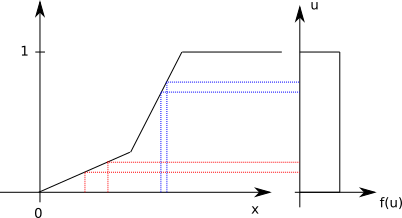
\includegraphics[scale=1.0]{images/generating_rvs.png}
\end{figure}


A high probability $f_X$ causes a steep cdf $F_X(x) = \int_{-\infty}^x f_X(u) du$ (in the same interval). This causes a large interval of $u$-values to be mapped onto a small interval of $x$-values, thereby causing a lot of ``probability'' to concentrate in this $x$-interval. This is illustrated in blue in the Figure. 

The opposite case of a smaller probability, causing a flatter cdf and less probability concentration on the same interval is shown in red in the Figure.

\subsection{Example - Asymmetric Triangluar Distribution}

Let's start with a asymmetric triangular distribution,

\bee
f_X(x) = \begin{cases} \frac{2}{a^2}x \quad & 0 \leq x \leq a \\
  0 \quad & \text{otherwise}
  \end{cases}
\eee

The corresponding cdf becomes

\bee
F_X(x) = \int_0^x \frac{2}{a^2}u du = \frac{x^2}{a^2} \quad 0 \leq x \leq a
\eee

The corresponding transform; i.e. the inverse cdf is then

\bee
T(u) = F_X^{-1}(u) = \sqrt{a^2 u}
\eee

If we take samples from a uniform RV in $[0,1]$ and plug them into this transform, the resulting $x = T(u)$ will have an asymmetric triangular distribution. \qed

\subsection{Example - (Truncated) Power-law Distribution}

This is the correction of \ref{2017-12-01:entry}. We start with the pdf of the truncated power-law distribution,

\bee
f(x) = \begin{cases}
	\frac{\alpha-1}{x_{\text{min}}} \left(\frac{x}{x_{\text{min}}}\right)^{-\alpha} &\quad x \geq x_{\text{min}} \\
	0 &\quad \text {otherwise}
\end{cases}
\eee

The cdf $F_X(x)$ then becomes

\bee
F_X(x) = \int_{x_{\text{min}}}^x \frac{\alpha-1}{x_{\text{min}}} \left(\frac{u}{x_{\text{min}}}\right)^{-\alpha} du = (\alpha-1) x_{\text{min}}^{\alpha-1} \int_{x_{\text{min}}}^x u^{- \alpha} du = (\alpha-1) x_{\text{min}}^{\alpha-1} \left. \frac{u^{-\alpha+1}}{-\alpha+1} \right|_{x_{\text{min}}}^x
\eee

Some further (tedious) messing around yields

\bee
F_X(x) = 1 - \left( \frac{x}{x_{\text{min}}} \right)^{-\alpha+1}
\eee

A quick sanity check: At $x = x_{\text{min}}$, the cdf becomes $F_X(x_{\text{min}}) = 0$ and for $x \rightarrow \infty$, the cdf approaches $1$ (for $\alpha > 1$).

Inverting the cdf and expressing as $x = F^{-1}(u)$ yields

\bee
x = x_{\text{min}} (1-u)^{1/(1-\alpha)}
\eee

This is the same result as \eqref{2017-12-01:eq1}. \qed

%%% Local Variables:
%%% mode: latex
%%% TeX-master: "journal"
%%% End:
